% Week 5 实验周报 —— 编译方式:XeLaTeX
\documentclass[11pt]{ctexart}
\usepackage[a4paper, margin=2.5cm]{geometry}
\usepackage{amsmath}
\usepackage{booktabs}
\usepackage{graphicx}
\usepackage{hyperref}
\usepackage{enumitem}
\setlist{nosep}

\title{\textbf{Chooser Option 定价项目 —— 第 5 周实验报告}\\
\large ML Model Design \& Implementation}
\author{佟铸城 (Zhucheng Tong)}
\date{2026 年 8 月 18 日}

\begin{document}
\maketitle

\section{本周目标}
完成 Week 5 三项交付物:(1) ML 架构设计文档;(2) 特征工程适配代码;(3) 两条路线的初版模型框架。

\section{完成工作}
\begin{enumerate}
  \item \textbf{数据管道}(\texttt{src/ml/dataset.py}):70/15/15 时序切分 + \textbf{净化}(训练尾部删 252 行,杜绝标签前视窗越界)+ 分模型族的特征适配(线性:16 特征标准化;树:18 原始特征;LSTM:63 日序列);
  \item \textbf{模型框架}(\texttt{src/ml/frameworks.py}、\texttt{lstm.py}):路线 A 四模型(Ridge/RF/GBDT/LSTM)+ 路线 B 三模型(Ridge/GBDT/MLP)+ 锚定变体三模型,统一训练入口,固定种子全确定;
  \item \textbf{纪律}:测试集本周不开封(第 6 周调参定型后只打开一次),所有结论基于验证集;
  \item \textbf{评估同尺}:沿用第 4 周 8 指标 + 加权综合分(参照 = 同期 EWMA 基线)。
\end{enumerate}

\section{核心实验结果:失败诊断与设计修正}
\begin{enumerate}
  \item \textbf{初版(直接预测波动率水平)全军覆没}:七个模型综合分 2.0--3.7(MLP 外推失稳达 90),全体正偏差 $+14$ 至 $+26$ 美元。诊断:训练窗被 COVID/2022 熊市主导,验证窗(2023--24)为低波动状态——树模型无法输出低于训练所见的值,线性/NN 被利率等特征的分布漂移带偏。\textbf{这不是调参能解决的问题,是目标参数化的设计缺陷};
  \item \textbf{设计修正——锚定目标}:改预测 $\ln(\sigma_{oracle}/\sigma_{EWMA})$,还原时 $\hat\sigma=\sigma_{EWMA}e^{\hat y}$。模型输出 0 即精确还原 EWMA 基线(已写成逐日审计断言),状态漂移被锚吸收,ML 只学``修正量'';
  \item \textbf{锚定 Ridge 成为首个击败基线的模型}(验证集):综合分 \textbf{0.567},定价 MAE \$3.90(基线 \$6.44,$-39\%$),Bias $-0.46$(初版 $+14$),$R^2$ 从基线 $-1.87$ 拉至 $-0.07$,Hit10 从 19.4\% 升至 35.2\%;波动率预测 MAE 3.8 个点(EWMA 持续性 6.0 个点);
  \item \textbf{诚实的另一面}:锚定未拯救树模型(3.8--4.2)——2023--24 的利率水平(5\%)在训练分布(\,$\leq2.5\%$)之外,树模型落入错误叶节点。修正方向明确:滚动重训 + 利率水平特征改为变化量特征(第 6 周);
  \item 与第 2 周重要性分析的呼应:锚定 Ridge 的头部系数是 VIX 系与波动率期限结构特征——前瞻信息对``修正量''的贡献与当时的探索性结论一致。
\end{enumerate}

\begin{figure}[h!]
\centering
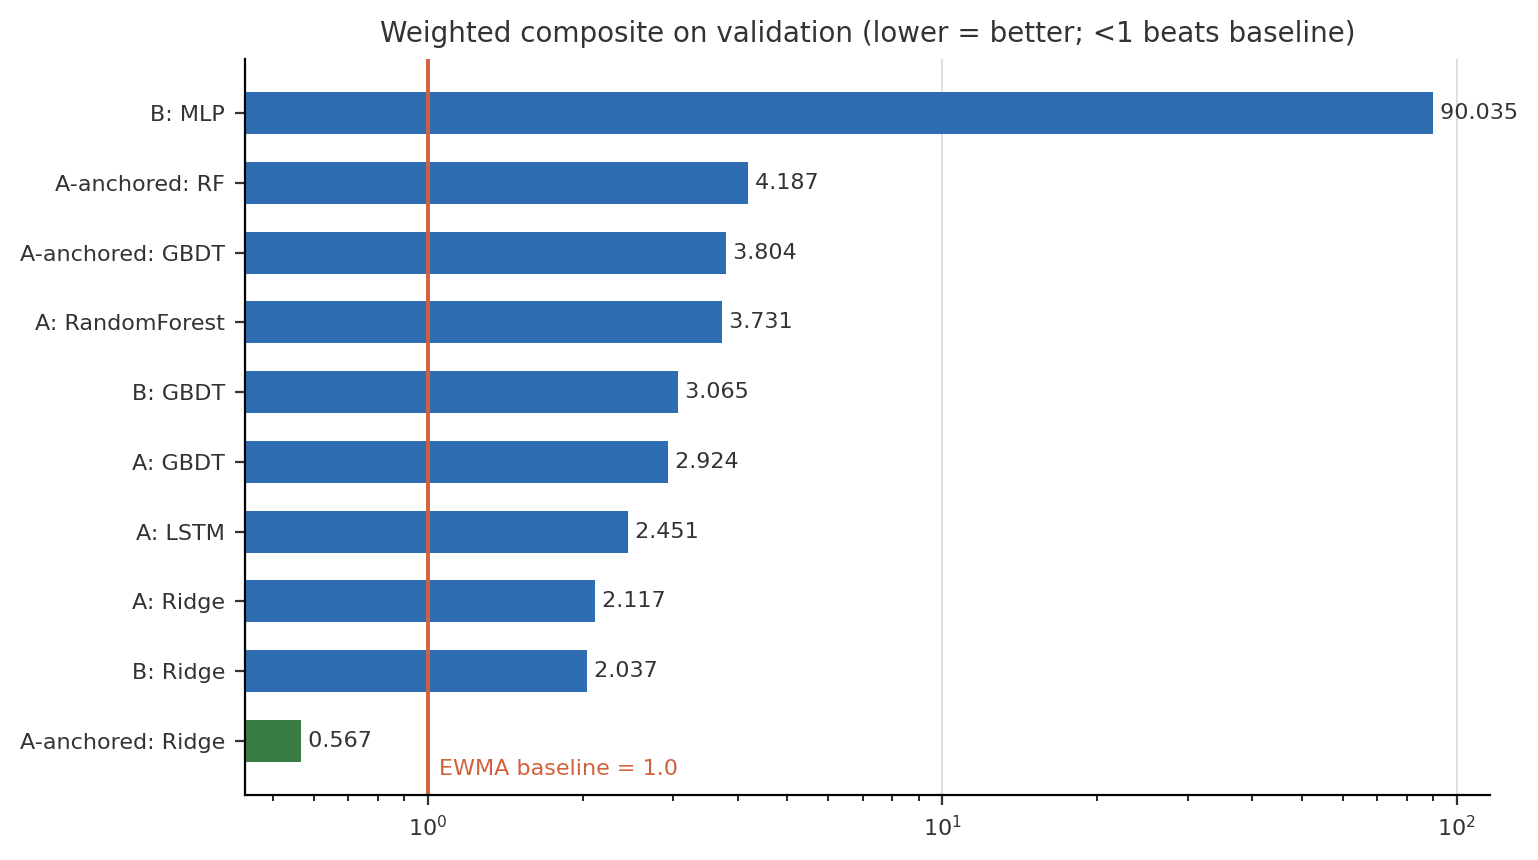
\includegraphics[width=0.78\textwidth]{../../docs/week5/figures/val_composite.png}
\caption{验证集加权综合分(对数轴,绿色 $<1$ 为胜过 EWMA 基线)}
\end{figure}

\section{实验记录}
一个方法论记录:初版七模型集体失败时,第一反应是查代码——六项审计(净化间隔、scaler 泄漏、锚定恒等式、测试集封存、重训确定性、综合分重算)全部通过后,才能把失败归因于设计而非实现。\textbf{排除 bug 是把失败转化为发现的前提};锚定修正的思想与第 3 周条件 MC 同源——把已知结构从任务中剥离,把学习留给残差。

\section{下周计划(Week 6:训练、调参与最终对比)}
walk-forward 滚动重训、利率特征改造、时序 CV 超参搜索、MLP 鲁棒化、锚定推广到路线 B;调参定型后\textbf{一次性开封测试集},输出 8 指标 + 综合分终表与 SHAP 可解释性分析。

\end{document}
